\documentclass[a4paper]{article}

\usepackage[francais,english]{babel}
\usepackage[utf8]{inputenc}
\usepackage[T1]{fontenc}
\usepackage{graphicx}
\usepackage{hyperref}

\usepackage[]{fullpage}

\makeatletter
\def\thickhrulefill{\leavevmode \leaders \hrule height 1pt\hfill \kern \z@}
\def\maketitle{%
  \null
  \thispagestyle{empty}%
  \vskip 1cm
  \begin{flushright}
        \normalfont\Large\@author
  \end{flushright}
  \vfil
  \hrule height 2pt
  \par
  \begin{center}
        \huge \strut \@title \par
  \end{center}
  \hrule height 2pt
  \par
  \vfil
  \vfil
  \null
\begin{center}
\Huge{Placement constraints for a better QoS in clouds}
\end{center}
\begin{figure}[!ht]
        \centering
        
\includegraphics[scale=.45]{imgs/cloud.png}
\end{figure}
\vfil
\begin{figure}[!ht]
        \centering
        \begin{minipage}[c]{.46\linewidth}
                
\includegraphics[scale=.3]{imgs/inria.png}
        \end{minipage}
        \begin{minipage}[c]{.2\linewidth}
                
\includegraphics[scale=.5]{imgs/polytech.png}
        \end{minipage}
\end{figure}
\vfil
\begin{description}
        \item[Entreprise] Université de Nice-Sophia Antipolis (INRIA)
        \item[Lieu] Sophia-Antipolis, France
        \item[Responsable] Fabien Hermenier, équipe OASIS,
        	\href{mailto:fabien.hermenier@unice.fr}{fabien.hermenier@unice.fr}
\end{description}
\cleardoublepage
}
\makeatother
\author{Mathieu Bivert, CSSR, \href{mailto:bivert@essi.fr}{bivert@essi.fr}}
\title{PFE: Cahier des charges (DOW)}

\begin{document}
\maketitle

\selectlanguage{francais}
\begin{abstract}
Blablabla français
\end{abstract}

\selectlanguage{english}
\begin{abstract}
Blablabla english
\end{abstract}

\tableofcontents
\newpage
\section{Description du projet}
\subsection{Contexte de travail}
Le monde industriel étant de plus en plus informatisé, la qualité des
réseaux s'améliorant, les sociétés informatiques tendent à ne vendre plus
de logiciels et de matériels mais louent des structures informatiques.

Les entreprises de services informatiques sont spécialisées dans la
maintenance de ces structures, donc par exemple plus performante
qu'une société de l'industrie automobile. Celle-ci peut donc choisir de
déporter donc la charge et paye pour une assurance sur la qualité du
service (QoS).

Plusieurs types d'entreprises existent selon le service qu'elles
proposent:
\begin{description}
	\item[SaaS] Software As A Service;
	\item[PaaS] Platform As A Service;
	\item[IaaS] Infrastructure As A Service;
	\item[DaaS] Data As A Service;
	\item[] $\ldots$
\end{description}

En particulier, un cloud \textit{IAAS} fournit à l'utilisateur l'accès
à un ensemble de systèmes d'exploitations. Ces derniers sont très
souvent virtualisés, ce qui présente l'avantage de pouvoir faire tourner
plusieurs OS sur un même serveur physique. Par exemple, la figure
\ref{hubertfxen} montre l'hyperviseur \textit{Xen} en train de faire
tourner, en plus d'un dom$0$ sous NetBSD, un FreeBSD, deux NetBSDs et
une Debian:
\begin{figure}[!ht]
	\centering
	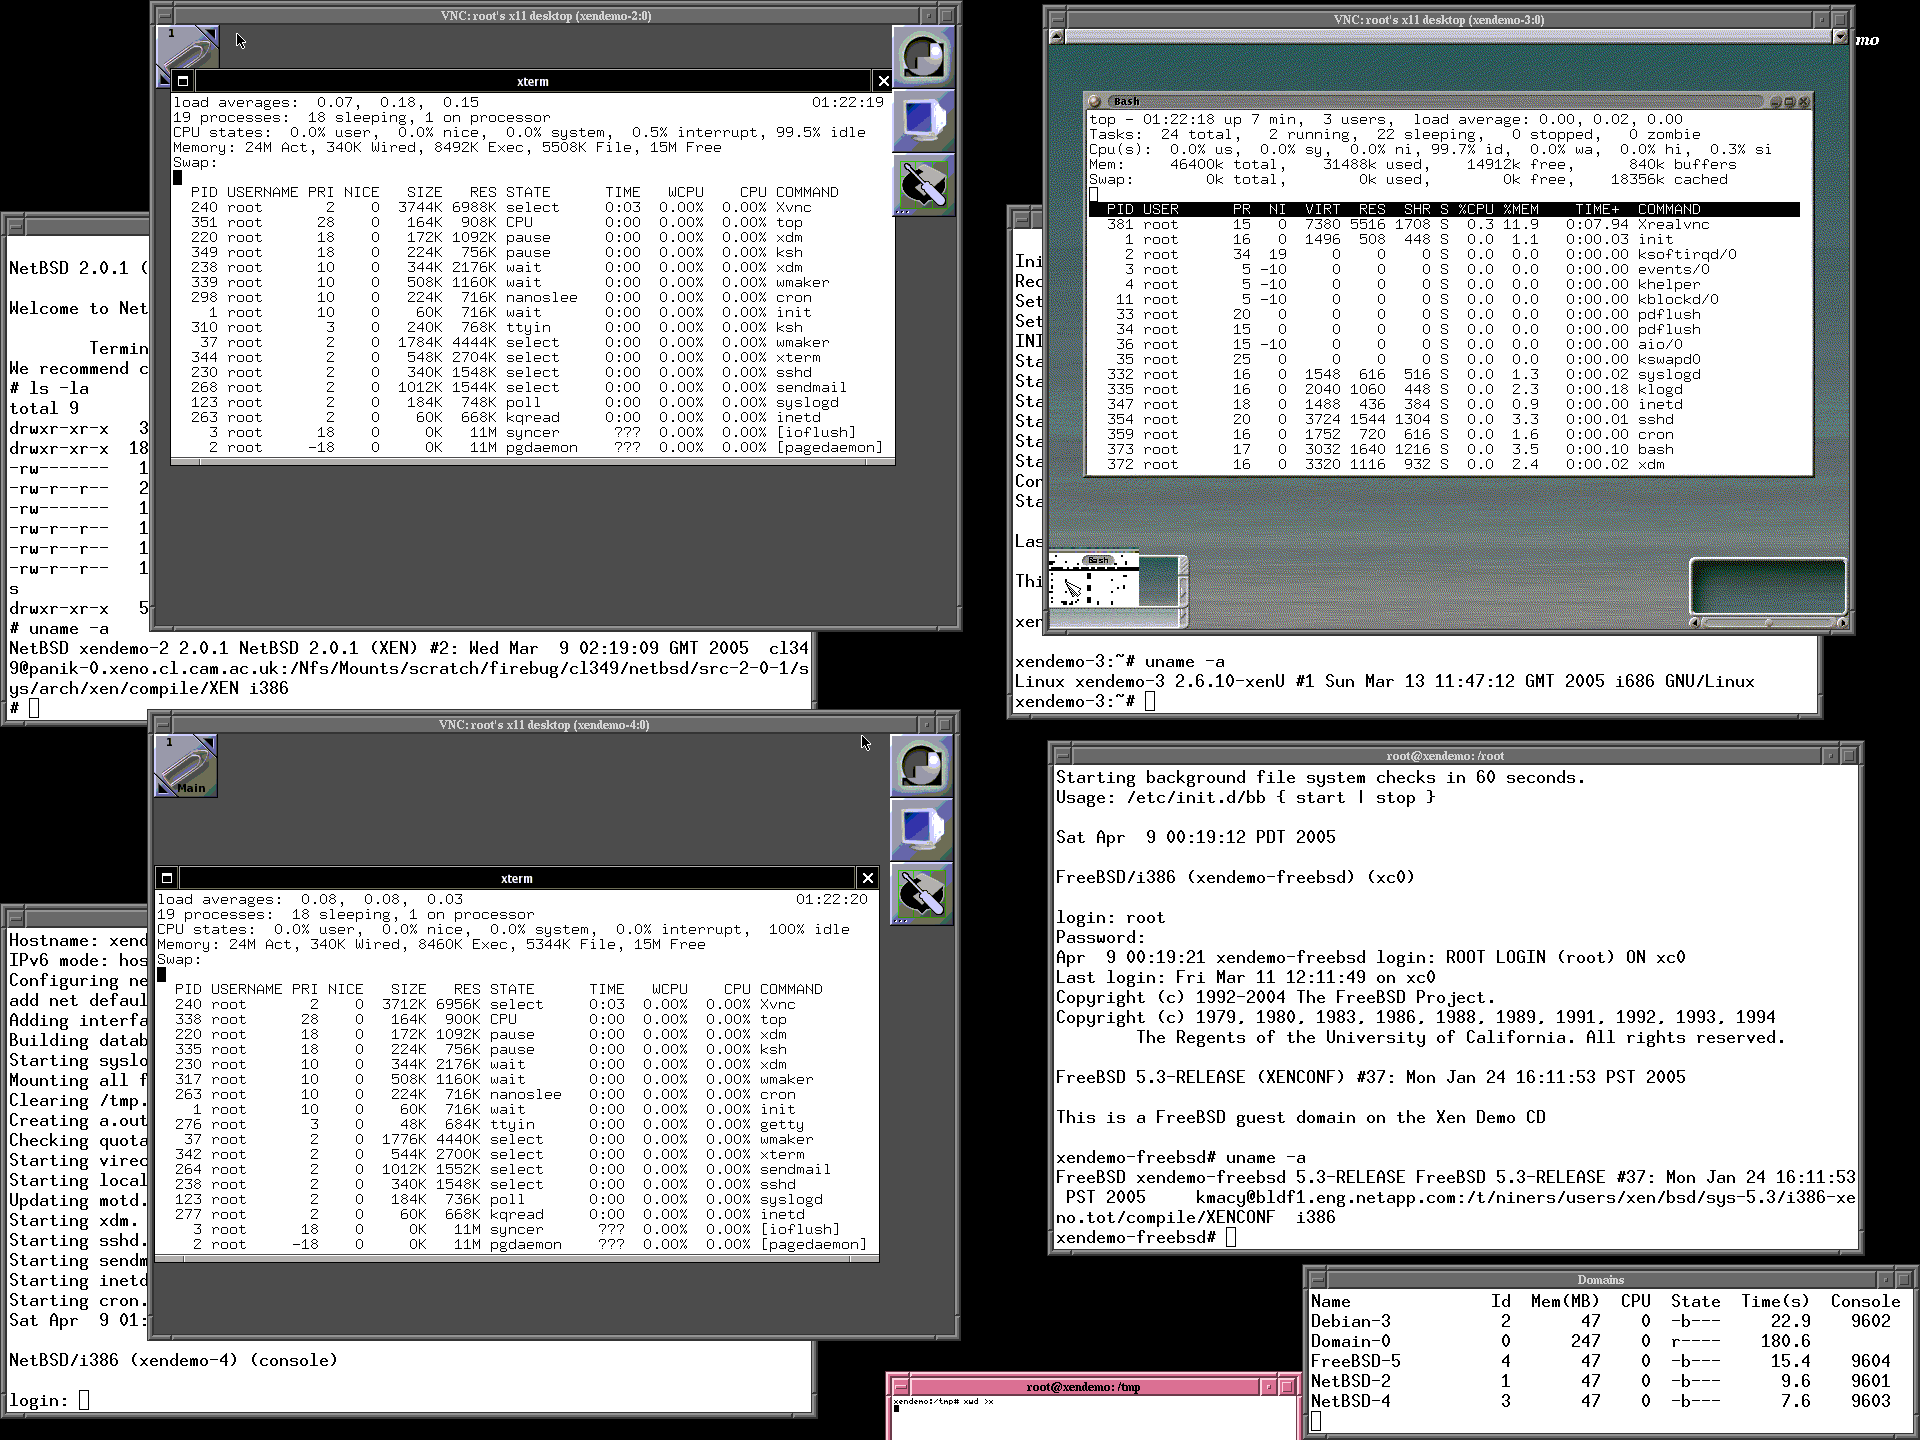
\includegraphics[scale=.2]{imgs/hubertf-xen.png}
	\caption{\label{hubertfxen} Virtualisation avec Xen}
\end{figure}

La virtualisation a plusieurs avantages:
\begin{itemize}
	\item sur une application dites $n$-tiers, il est possible
	de placer chaque tiers sur une VM, et éventuellement d'en faire
	des duplications, ce qui améliore la robustesse de l'application;
	\item l'admninistration et la gestion des machines est simplifiée :
	il y a moins de hardware, donc moins de maintenance physique;
	\item chaque application peut être répartie sur une VM différente.
	Ainsi, si une application est compromise, elle a moins de chances
	de pouvoir compromettre d'autres applications que si elles étaient
	toutes lancées sur une même machine physique.
	\item utilisation plus performante du matériel : on est plus dans
	le cas où dans une entreprise, des dizaines de postes de Bureau
	\og assez \fg puissants sont tous utilisés en même temps à quelques
	dixième de leur capacité totale;
	\item $\ldots$
\end{itemize}

Une problématique pour les gestionnaires d'IAAS est donc de pouvoir placer
correctement un ensemble donné de VMs $\mathcal{V}$ sur un ensemble de
serveurs physiques $\mathcal{N}$.

\subsection{Motivations}
La question de la répartition des machines virtuelles sur les machines
physiques se pose alors pour des raisons diverses et variées:
\begin{description}
	\item[maintenance] un serveur physique peut tomber en panne, ou
		nécessiter une réparation, auquel cas les programmes
		tournant dessus doivent être migré ailleurs, afin de
		garantir au client une certaine qualité de service (QoS);
	\item[sécurité] il peut s'avérer risquer pour un programme d'un
		client traitant des données sensibles (eg. données bancaires)
		de se retrouver au même endroit qu'un programme d'un
		autre client;
	\item[évolution des besoins] où au cours d'un certain intervalle de
		temps, les besoins en puissance de calcul d'une entreprise
		peuvent augmenter (suite à une plus grande popularité par
		exemple), ou encore, augmentation brusque et irrégulière
		de la charge à des heures de pointes;
	\item[économie d'énergie] où il peut être avantageux de réduire
		le nombre de serveurs physiques allumés, pour maximiser
		le rendement des autres machines physiques du cloud;
	\item[QoS] où, à l'inverse de l'économie d'énergie, il est bon
		de garder des ressources supplémentaires disponibles immédiatement,
		de façon a ne pas perdre de temps (et donc en QoS) à redémarrer
		un autre serveur;		
	\item[licence] les entreprises fournissant les systèmes de virtualisation
		proposent des licences selon différents critères (eg. nombre de
		machines virtuelles lancées, utilisation de ressources (CPU, RAM, etc.));
	\item[plateforme] plusieurs plateformes de virtualisations sont disponibles
		(eg. Xen, VMWare, Citrix); une autre contrainte sur la
		répartition des machines virtuelles se pose alors, un serveur
		physique ne faisant tourner qu'un seul type de plateforme;
	\item[] $\ldots$
\end{description}
\subsection{Défis}
Afin de pouvoir répondre aux besoins exprimés par l'un des domaines
cité dans le paragraphe précédent, il est nécessaire de commencer
par formaliser le problème. En d'autres termes, donner une définition
mathématiques des contraintes impliquées par la problèmatique choisie,
et s'assurer qu'elles sont envisageables en pratique. Finalement, cette
représentation abstraite doit être implémentée sous forme de plugin
Java pour entropy~\cite{herm2009} un manager de clusters reposant sur
l'algorithme btrplace\footnote{\url{http://btrp.inria.fr/sandbox/about.html}}.

\subsection{Objectifs}
Actuellement, les trois derniers points cités ne sont pas forcément
formalisé/implémenté sous une forme satisfaisante. Le projet consiste
donc à choisir l'un de ces domaines et à l'ammener vers une forme
satisfaisante.

Le dernier point est celui sur lequel se porte ce projet.
\subsection{Scénarios}
\begin{figure}[!ht]
        \centering
        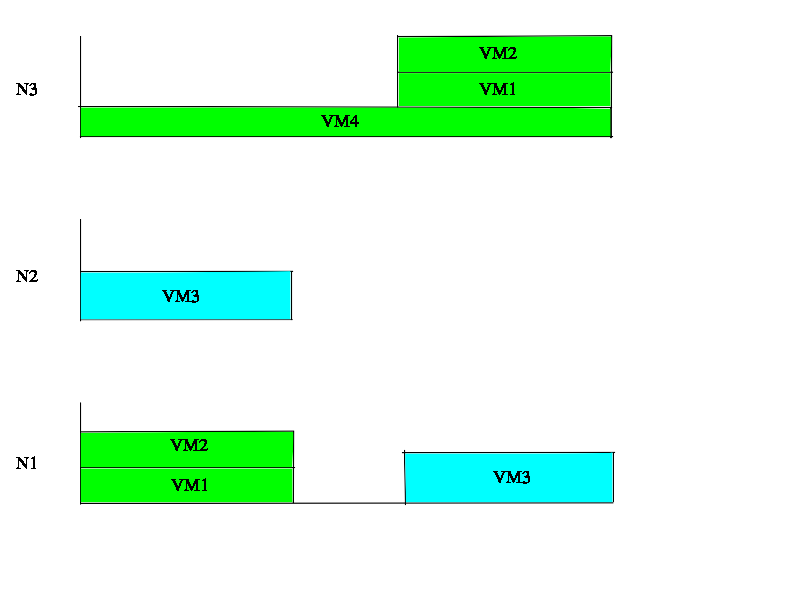
\includegraphics[scale=.3]{imgs/vmreconf.png}
	\caption{\label{usecase} Exemple de changement de système de virtualisation. En vert des VMs Xen, en cyan une VM VMWare}
\end{figure}

Sur le diagramme ci dessus, le serveurs physiques $N_2$ doit êtres mis
hors-ligne pour des questions de maintenance, via la contrainte
\textit{offline($N_i$);}\footnote{\url{http://www-sop.inria.fr/members/Fabien.Hermenier/btrpcc/offline.html}}.

Comme aucun serveur VMWare n'est disponible, il est nécessaire de supprimer
un serveur Xen, capable d'accueillir $VM_3$, par exemple $N_1$.

\subsection{Critère de succès}
bis repetita: trouver un bon formalisme; définir et implémenter
les contraintes.
\section{État de l'art}
\subsection{Description générale}
\subsection{foo}
\subsection{bar}

\section{Méthodologie et planification}
\subsection{Stratégie générale}
bis repetita: trouver un bon formalisme; définir et implémenter
\subsection{Découpage en lots}
bis repetita: trouver un bon formalisme; définir et implémenter
\subsection{Plannification}
gantt
\subsection{Livrables associés au projet}
\begin{table}
\centering
\begin{tabular}{c|c|c|c|c}
	Id & Titre du livrable & Lot(s) & Nature & Date \\
	\hline
	\hline
	$D_0$ & Cahier des charges & $1$ & Document & $S_4$ \\
	\hline
	$D_1$ & Gestion du typage et du déploiement & $1$ & Document & $?$ \\
	\hline
	$D_2$ & Ensemble de contraintes & $1$ & Document et Logiciel & $?$ \\
	\hline
	$D_3$ & Rapport de management & $1$ & Document & $S_{20}$ \\
	\hline
	$D_4$ & Diaporama de présentation finale & $1$ & Document & $S_{20}$ \\
\end{tabular}
\end{table}

\subsection{Jalons}
\begin{table}
\centering
\begin{tabular}{c|c|c|c|c}
	Id & Jalon de fin de phase & Lot(s) & Date & Vérification \\
	\hline
	\hline
	$J_0$ & planification & $1$ & $S_4$ & $D_0$ \\
	\hline
	$J_1$ & formalisation & $1$ & $S_n$ & $D_1$ partiel \\
	\hline
	$J_2$ & implémentation & $1$ & $S_{n+k}$ & $D_2$, $D_1$ partiel \\
	\hline
	$J_3$ & projet & $1$ & $S_{20}$ & $D_1$, $D_2$, $D_3$ et $D_4$ \\
\end{tabular}
\end{table}

\section{Description de la mise en œuvre du projet}
\subsection{Interdépendance des lots et tâches}
bis repetita: trouver un bon formalisme; définir et implémenter
\subsection{Description des lots}
bis repetita: trouver un bon formalisme; définir et implémenter
\subsection{Résumé de l'effort}
\subsection{Gestion du risque}

\section{Participants}
\subsection{Mathieu Bivert - CSSR}
Étudiant à Polytech'Nice Sophia, spécialisé en Cryptographie, Systèmes
Sécurité et Réseaux.

\subsection{Fabien Hermenier - OASIS/INRIA}
\textbf{Fabien Hermenier} a recu un doctorat en $2009$ à l'université
de Nantes. Depuis $2011$, il enseigne en tant que professeur adjoint
à l'université de Nice Sophia-Antipolis. Son travail de recherche
s'articule autour des plateformes d'hébergement, de la virtualisation,
du calcul autonome et de la gestion des ressources. Depuis $2006$, il
travaille sur des algorithmes de placement de machines virtuelles pour
faire face à l'augmentation des SLA dans les plateformes d'hébergements.

\newpage
\selectlanguage{francais}
\bibliographystyle{alpha}
\bibliography{docs}

\end{document}

